\RequirePackage[l2tabu, orthodox]{nag}
\documentclass[11pt,uplatex]{jsarticle}

\usepackage[dvipdfmx]{graphicx}
%\usepackage{verbatimfiles}
\usepackage{multicol}
\usepackage{mathptmx}
\usepackage{color}
\usepackage{lscape}
\usepackage{amsmath}
% % \usepackage{dcolumn}

%\usepackage{a4jm}
%\usepackage{subeqn}
\usepackage[margin=1in]{geometry}


\def\d#1#2{\frac{d #1}{d #2}}
\def\dd#1#2{\frac{d^2 #1}{d #2^2}}
\def\pd#1#2{\frac{\partial #1}{\partial #2}}
\def\pdd#1#2{\frac{\partial^2 #1}{\partial #2^2}}
\def\Ene{\varepsilon}
\def\DOS{\mathcal{D}}
\def\vec#1{{\bm{#1}}}
\def\kvec{\bm{k}}
\def\kvecp{{\bm{k}'}}
\def\subvec#1{{\boldsymbol{\small #1}}}
 
\def\GP{{\vec{G}_\parallel}}
\def\GPP{{\vec{G}^\prime_\parallel}}
\def\KP{{\vec{k}_\parallel}}
\def\KP{{\vec{k}_\parallel}}
\def\XP{{\vec{x}_\parallel}}

\def\EneK{\varepsilon_{\kvec}}
\def\EneKp{\varepsilon_{\kvec^{'}}}
\def\EneKn{\varepsilon_{\kvec n}}
\def\EneKnp{\varepsilon_{\kvec^{'} n^{'}}}
\def\EneKm{\varepsilon_{m \vec{k}}}
\def\EneKmp{\varepsilon_{m' \vec{k}'}}

\def\bra#1{{\langle #1 |}}
\def\ket#1{{| #1 \rangle}}
\def\braket#1#2{{\langle #1 | #2 \rangle}}
\def\av#1{{\langle #1 \rangle}}

\def\sinc{\mathrm{sinc}}
\def\sgn{\mathrm{sgn}_{n,p}}
\def\Tr{{\mathrm{Tr}\, }}

\def\Ene{\varepsilon}
\def\vec#1{{\bf #1}}
\def\taumue{{\langle \tau\rangle}}
\def\tauH{{\langle \tau^H \rangle}}
\def\GP{{\vec{G}_\parallel}}
\def\GPP{{\vec{G}^\prime_\parallel}}
\def\KP{{\vec{k}_\parallel}}
\def\KP{{\vec{k}_\parallel}}
\def\XP{{\vec{x}_\parallel}}

\def\vvec#1{{\bf #1}}

\def\Ene{\varepsilon}
\def\vec#1{{\bf #1}}
\def\taumue{{\langle \tau\rangle}}
\def\tauH{{\langle \tau^H \rangle}}
\def\GP{{\vec{G}_\parallel}}
\def\GPP{{\vec{G}^\prime_\parallel}}
\def\KP{{\vec{k}_\parallel}}
\def\KP{{\vec{k}_\parallel}}
\def\XP{{\vec{x}_\parallel}}

\def\vvec#1{{\bf #1}}

\begin{document}
\title{Cylindrical MESFET/MOSFET}
\author{J.~Motohisa\\Graduate School of IST, Hokkaido University}
\maketitle

\section{Cyrlindircal MESFET}
\subsection{Poisson Equation}
Poisson方程式
\begin{equation}
 \frac{1}{r} \d{}{r}(r\d{\psi}{r}) = \frac{q}{\epsilon} N_D
\end{equation}
の一般解は
\begin{equation}
\psi(r) = -\frac{q N_D}{4 \epsilon }r^2 +c_1 \ln r + c_2
\end{equation}
であり、境界条件は空乏層幅を$W$として
\begin{eqnarray}
 \psi(R-W)&=&0 \\
 \left. \d{\psi}{r}\right|_{r=R-W}&=&0\\
 \psi(R)&=&-V_{bi}
\end{eqnarray}
$\tilde{R}=(R-W)/R$とおくと
\begin{eqnarray}
c_1 &=& \frac{q N_D}{2 \epsilon} \tilde{R}^2 \\
c_2& =& \frac{q N_D}{4 \epsilon}\tilde{R}^2 (1-\ln (R^2\tilde{R}^2))
\end{eqnarray}
\begin{equation}
 \frac{4 \epsilon}{e N_D R^2} V_{bi} = (1-\tilde{R}^2)+\tilde{R}^2 \ln \tilde{R}^2\label{eqn:R}
\end{equation}
式(\ref{eqn:R})の右辺をプロットしたものを図\ref{fig:rgraph}に示す。

\begin{figure}[htbp]
 \begin{center}
  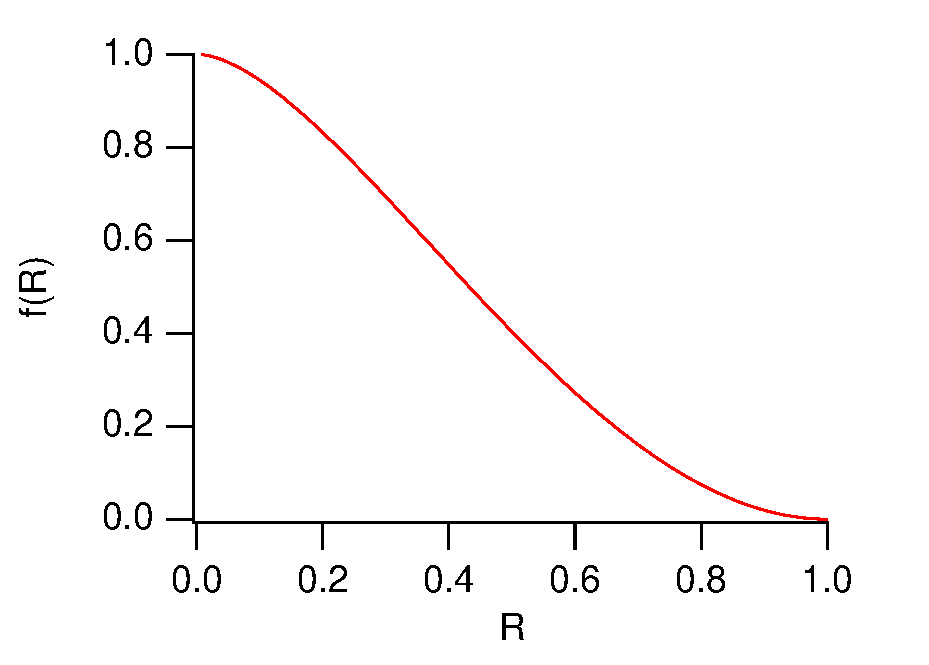
\includegraphics[width=8cm,keepaspectratio]{Rgraph.eps}
  \caption{式(\protect{\ref{eqn:R})}の右辺を$R$の関数としてプロットした
  グラフ\label{fig:rgraph}}
  \end{center}
 \end{figure}

\subsection{Gradual Channel Approximation}
Gradual Channel Approximationでは式(\ref{eqn:R})において$V_{bi}\to
V_{bi}-V_{GS}+V(x)$と置き換える。
MESFETのしきい値は$V(x)=0$のとき$\tilde{R}=0$となるゲート電圧であり、
\begin{equation}
 V_{th}=V_{bi}-\frac{q N_D R^2}{4 \epsilon}
\end{equation}
となる。

$V_{GS}>V_{th}$のとき、電流は
\begin{equation}
 I_{DS}=e (N_D \pi R^2 \tilde{R}^2) \mu \d{V}{z}
\end{equation}
より積分して
\begin{equation}
 I_{DS}=\frac{\pi q N_D R^2 \mu}{L}\int_0^{V_{DS}} \tilde{R}^2 dV
\end{equation}
さて
\begin{equation}
 \int_0^{V_{DS}} dV = \int_{R_S}^{R_D} \d{V}{\tilde{R}} d\tilde{R}
\end{equation}
であり、また式(\ref{eqn:R})より
\begin{equation}
 \d{V}{\tilde{R}} = \frac{q N_D R^2}{\epsilon} \tilde{R} \ln\tilde{R}
\end{equation}
であるから
\begin{equation}
I_{DS} = K \{\tilde{R}_S^4(1-\ln \tilde{R}_S^4)\} - \tilde{R}_D^4(1-\ln\tilde{R}_D^4)\}\label{eqn:ids}
\end{equation}
ここで
\begin{equation}
 K=\frac{\pi e^2 N_D^2 R^4}{16 L \epsilon}
\end{equation}
また$\tilde{R}_S$、$\tilde{R}_D$はそれぞれソース端・ドレイン端での中性領
域の規格化した半径であり、式(\ref{eqn:R})より求められる。
\section{Transconductance}
式(\ref{eqn:ids})を$V_{GS}$で微分すると、
\begin{equation}
 \d{\tilde{R}}{V_{GS}} = - \frac{\epsilon}{q N_D R^2} \frac{1}{\tilde{R}
  \ln \tilde{R}}
\end{equation}
であるので、相互コンダクタンス
\begin{equation}
 g_m =\d{I_{DS}}{V_{GS}}= \frac{\pi e N_D \mu R^2}{L} (\tilde{R}_S^2 - \tilde{R}_D^2)
\end{equation}
この式は飽和領域で$\tilde{R}_D=0$とすれば、線形領域、飽和領域のいずれで
も成立する。

\section{MOSFET}
\subsection{Poisson Equation}
Poisson方程式は
\begin{equation}
 \frac{1}{r} \d{}{r}(r\d{\phi}{r}) =  \frac{q n_i}{\epsilon} \exp\left(\frac{q(\phi-V)}{k_B T}\right)
\end{equation}
境界条件は
\begin{eqnarray}
 \phi(R)&=&\phi_s \\
\left. \d{\phi}{r}\right|_{r=0}&=&0
 \end{eqnarray}
\begin{equation}
 L_D = \sqrt{\frac{k_B T \epsilon}{q^2 n_i}}
\end{equation}
を用いて
\begin{equation}
 \tilde{r}=r/L_D
\end{equation}
および
\begin{equation}
 y=\exp\left[ -\frac{q(\phi-V)}{k_B T} \right]
\end{equation}
と置くと微分方程式
\begin{equation}
\frac{1}{\tilde{r}} \d{}{\tilde{r}}\frac{\tilde{r}y'}{y} = \frac{1}{y}
\end{equation}
を得る。この方程式の解のひとつは
\begin{equation}
 y=(C + \tilde{r}^2)^2/8C
\end{equation}

\section{Poisson Equation (2)}
Poisson方程式は
\begin{equation}
 \frac{1}{r}\d{}{r}(r\d{\phi}{r}) =  -\frac{q}{\epsilon}
  (N_D^ + p - N_A^- - n)
\end{equation}
電荷中性条件
\begin{equation}
 N_D^+ - N_A^- = n_{p0}-p_{n0}
\end{equation}
および
\begin{equation}
 n=n_{p0} \exp(\beta \phi),\ p = p_{p0} \exp(-\beta\phi)
\end{equation}
を使って
\begin{equation}
 \frac{1}{r}\d{}{r}(r\d{\phi}{r})
  =-\frac{q}{\epsilon_{\mathrm{S}}}
[p_{p0}(e^{-\beta \phi} -1) - n_{p0} (e^{\beta \phi} -1)]
\end{equation}
これを$\phi$について積分すると左辺は
\begin{subequations}
\begin{align}
\int \frac{1}{r}[\d{}{r}(r \d{\phi}{r})]d\phi
  & =
  \int \frac{1}{r}[\d{}{r}(r \d{\phi}{r})]\d{\phi}{r} dr
  =\int (\dd{\phi}{r})\d{\phi}{r} d r +
  \int \frac{1}{r}(\d{\phi}{r})^2 dr \\
&= \frac{1}{2}(\d{\phi}{r})^2 + C + \int \frac{1}{r}(\d{\phi}{r})^2 dr 
\end{align}
\end{subequations}


\end{document}



